% main. Внутри функции main

\chapter{Внутри функции main}

Как вы знаете, каждая программа на C начинается с выполнения функции с именем main, которая вызывается из функции запуска в среде выполнения C. Основная функция будет вызывать другие функции (подфункции) для выполнения большей части обработки. Даже простое <<\code{Hello, World!}>> программе необходимо вызвать другую функцию, чтобы вывести сообщение на экран.

Большинству подфункций требуется, чтобы данные передавались им в качестве аргументов от вызывающей функции, и они часто передают результат обратно вызывающей функции. Аргументами функции могут быть данные или адреса памяти. Когда функция вызывается, она выполняет свои операции, а затем возвращается к вызывающей функции. Вызывающая функция должна отправить вызываемой функции адрес для возврата. В архитектуре x86-64 адрес возврата передается в стеке вызовов.

Добавляя немного сложности, большинству функций нужны свои собственные локальные переменные для хранения данных и адресов. Регистры можно использовать для переменных, но они глобальны, и нам быстро не хватит регистров для использования. Стек обеспечивает хорошее место для выделения места для локальных переменных в памяти.

В этой главе мы разберем этот процесс. Мы сделаем это, обсудив, как писать символы на экране и читать символы с клавиатуры в нашей основной функции. Начиная с этой главы, мы обычно обходим функции стандартной библиотеки C, printf и scanf, и используем функции системного вызова write для вывода на экран и read для ввода с клавиатуры.

Мы начнем с обсуждения функций записи и чтения. Затем мы рассмотрим, как аргументы передаются функции в регистрах процессора. Далее мы рассмотрим, как ЦП может определить адрес для передачи функции, когда это необходимо. Затем мы рассмотрим, как структура данных, называемая стеком вызовов, используется для создания локальных переменных внутри функции.

\section{Функции системного вызова записи и чтения}

В главе 2 мы использовали \code{printf} и \code{scanf} из стандартной библиотеки C для записи на экран и чтения с клавиатуры. Как показано на рис. 2-1 (в главе 2), \code{printf} преобразует данные из формата хранения в памяти в символьный формат и вызывает функцию системного вызова \code{write} для отображения символов на экране. При чтении символов с клавиатуры \code{scanf} вызывает функцию системного вызова \code{read} и преобразует символы в формат хранения в памяти.

Linux видит экран и клавиатуру как файлы. При первом запуске программы операционная система открывает три файла — стандартный ввод, стандартный вывод и стандартный файл ошибок — и присваивает каждому файлу целое число, называемое файловым дескриптором. Программа взаимодействует с каждым файлом, используя файловый дескриптор. Интерфейсы C для вызова операций чтения и записи указаны в стандарте Portable Operating System Interface (POSIX). Общие форматы для вызова этих двух функций:

\begin{ffcode}
int write(int fd, char *buf, int n);
int read(int fd, char *buf, int n);
\end{ffcode}
где \code{fd} — дескриптор файла, \code{buf} — адрес хранилища символов, а \code{n} — количество символов для чтения или записи. Вы можете увидеть более подробную информацию в справочных страницах для записи и чтения:

\begin{ffcode}
man 2 write
man 2 read
\end{ffcode}

В таблице~\ref{table-descriptors} показаны дескрипторы файлов, которые мы будем использовать, и устройства, с которыми каждый из них обычно связан.

\begin{table}[h]
    \caption{Дескрипторы файлов для записи и чтения функций системного вызова}
    \centering
    \begin{tabular}{lll}
        \hline
        \textbf{Имя} & \textbf{Номер} & \textbf{Использование} \\ \hline \hline
        \rowcolor{lightgray}
        \verb|STDIN_FILENO| & 0 & Чтение символов с клавиатуры \\ 
        \verb|STDOUT_FILENO| & 1 & Вывод символов на экран \\ 
        \rowcolor{lightgray}
        \verb|STDERR_FILENO| & 2 & Вывод ошибок на экран \\ \hline
    \end{tabular}
    \label{table-descriptors}
\end{table}

Эти имена определены в системном заголовочном файле \verb|unistd.h|, который находится в \verb|/usr/include/unistd.h| в моей системе Ubuntu. (Расположение в вашей системе может быть другим.)

Давайте посмотрим, как передать соответствующие аргументы функции записи для вывода текста на экран.

\section{Передача аргументов в регистрах}

В нашей среде можно передавать до шести аргументов в регистрах от одной функции к другой. Мы рассмотрим, как передавать более шести аргументов, в главе 14, и здесь я отмечу, что среда Windows C позволяет передавать в регистрах только четыре аргумента.

Начнем с программы, которая делает что-то очень простое. Мы напишем <<\code{Hello, World!}>> на экране с помощью функции системного вызова записи (листинг 11-1).

\begin{ffcode}
/* helloWorld.c
 * Hello World program using the write() system call.
 */

#include <unistd.h>

int main(void)
{

  write(STDOUT_FILENO, "Hello, World!\n", 14);

  return 0;
}
\end{ffcode}

\begin{center}
Листинг 11-1: «Привет, мир!» программа, использующая функцию системного вызова записи
\end{center}

Эта функция передает три аргумента для записи. В принципе, компилятор C — или вы, когда пишете на ассемблере, — можете использовать любой из 16 регистров общего назначения, кроме \code{rsp}, для передачи аргументов от одной функции к другой. (Причина, по которой вы не можете использовать \code{rsp}, будет объяснена чуть позже.) Просто сохраните аргументы в регистрах и вызовите нужную функцию. Конечно, компилятору или человеку, пишущему на ассемблере, необходимо точно знать, в каком регистре находится каждый аргумент, когда речь идет о вызываемой функции.

Лучший способ избежать ошибок — разработать стандартный набор правил и следовать им. Это особенно важно, если код для программы пишут несколько человек. Другие люди осознали важность наличия таких стандартов и предоставили хороший набор стандартов для передачи аргументов в приложении \textbf{System V Application Binary Interface AMD64 Architecture Processor Supplement} (с моделями программирования LP64 и ILP32) версии 1.0. Я нашел версию от 28 января 2018 года в формате PDF по адресу \code{https://github.com/hjl-tools/x86-psABI/wiki/x86-64-psABI-1.0.pdf}. (Последняя версия поддерживается в исходном коде LaTeX по адресу \code{https://gitlab.com/x86-psABIs/x86-64-ABI/}, но вам понадобится \code{pdflatex} для создания PDF-версии.) Используемый нами компилятор, gcc, следует правила стандартов System V, и мы сделаем то же самое для языка ассемблера, который мы пишем.

Табл. 11-2 суммирует стандарты System V для использования регистров.

\begin{table}[h]
    \caption{Использование регистров общего назначения}
    \centering
    \begin{tabularx}{\textwidth}{lXl}
        \hline
        \textbf{Регистр} & \textbf{Специальное применение} & \textbf{Сохранять?} \\ \hline \hline
        \rowcolor{lightgray}
        rax & Вернуть первое значение из функции & Нет \\
        rbx & общего назначения & Да \\
        \rowcolor{lightgray}
        rcx & Передать четвертый аргумент в функцию & Нет \\
        rdx & Передать третий аргумент в функцию; вернуть второе значение из функции & Нет \\
        \rowcolor{lightgray}
        rsp & указатель стека & Да \\
        rbp & Необязательный указатель кадра & Да \\
        \rowcolor{lightgray}
        rdi & Передать первый аргумент функции & Нет \\
        rsi & Передать второй аргумент в функцию & Нет \\
        \rowcolor{lightgray}
        r8 & Передать пятый аргумент функции & Нет \\
        r9 & Передать шестой аргумент функции & Нет \\
        \rowcolor{lightgray}
        r10 & Указатель статической цепочки функции Pass & Нет \\
        r11 & Нет & Нет \\
        \rowcolor{lightgray}
        r12 & Нет & Да \\
        r13 & Нет & Да \\
        \rowcolor{lightgray}
        r14 & Нет & Да \\
        r15 & Нет & Да \\
    \end{tabularx}
    \label{table-descriptors}
\end{table}

Столбец <<\textbf{Сохранить?}>> показывает, должна ли вызываемая функция сохранять значение в этом регистре для вызывающей функции. Вы узнаете, как это сделать, в следующих нескольких разделах.

Первые шесть аргументов передаются в регистрах \code{rdi, rsi, rdx, rcx, r8 и r9}, читаясь слева направо в функции C. В листинге 11-2 показан язык ассемблера, сгенерированный gcc для функции C в листинге 11-1. Это иллюстрирует, как передать три обязательных аргумента функции записи.

\textbf{Примечание.}
\textit{Компилятор не комментировал код на ассемблере в этом листинге. Я добавил свои собственные комментарии, используя <<\#\#>>, чтобы помочь вам увидеть взаимосвязь с исходным кодом C. Я проделаю это с большей частью языка ассемблера, сгенерированного компилятором, который я покажу в этой книге.}

\begin{ffcode}
	.file	"helloWorld.c"
	.intel_syntax noprefix
	.text
	.section	.rodata
.LC0:
	.string	"Hello, World!\n"
	.text
	.globl	main
	.type	main, @function
main:
	push	rbp
	mov	rbp, rsp
	mov	edx, 14
	lea	rax, .LC0[rip]
	mov	rsi, rax
	mov	edi, 1
	call	write@PLT
	mov	eax, 0
	pop	rbp
	ret
	.size	main, .-main
	.ident	"GCC: (GNU) 12.1.1 20220730"
	.section	.note.GNU-stack,"",@progbits
\end{ffcode}

Листинг 11-2: Язык ассемблера, сгенерированный gcc для программы в Листинге 11-1

При программировании на ассемблере принято хранить аргументы в регистрах, начиная с последнего аргумента в списке аргументов, продвигаясь к первому аргументу. В листинге 11.2 третий аргумент для записи, количество символов (3), сохраняется первым в регистре для третьего аргумента, \code{edx}. Второй аргумент — это адрес первого символа в строке (4), которая идет в \code{rsi}. Первый аргумент, устройство для записи в (5), хранится в \code{edi} непосредственно перед вызовом для записи (6).

Эта программа также вводит еще две инструкции, \code{lea} и \code{call}, и довольно странный синтаксис, связанный с этими инструкциями. Инструкция lea загружает адрес памяти \code{.LC0} в регистр \code{rsi}, а инструкция \code{call} передает управление программой на адрес функции записи. Прежде чем описывать детали этих инструкций, нам нужно посмотреть, где в памяти расположены различные компоненты программы.

\section{Позиционно-независимый код}

Задача компоновщика состоит в том, чтобы решить, где в памяти должен располагаться каждый программный компонент, а затем заполнить адреса в программном коде, где указан компонент. Компоновщик может решить, где каждый компонент должен быть расположен в памяти, и включить эти адреса в исполняемый файл, но более безопасно позволить операционной системе решить, где загрузить каждый компонент. Давайте посмотрим, как язык ассемблера, сгенерированный gcc, позволяет загружать программу в любом месте памяти.

Чтобы программа работала правильно, когда на операционную систему возложена обязанность решать, куда ее загрузить, компоновщик должен создать исполняемый файл, независимый от позиции. Чтобы это работало, каждая функция в программе должна состоять из независимого от позиции кода, кода, который будет работать правильно независимо от того, где он загружен в память. По умолчанию компилятор gcc обычно настроен на создание кода, не зависящего от позиции, а на этапе компоновки создается исполняемый файл, не зависящий от позиции.

Связать функции и глобальные элементы данных в файлах исходного кода, которые мы пишем для нашей программы, несложно. Компоновщик знает, сколько байтов содержится в каждой функции и глобальном элементе данных, поэтому он может вычислить, где каждый из них начинается относительно начала программы. Оттуда компоновщик может вычислить количество байтов от места ссылки на компонент до относительного местоположения компонента, на который делается ссылка, давая значение смещения. Компоновщик вставляет это значение смещения в код в том месте, где имеется ссылка на компонент.

Вы уже узнали о цикле выполнения и о том, как указатель инструкций перемещается по программе по мере ее выполнения. В результате в любой заданной точке программы текущий адрес находится в указателе инструкций, \code{rip}, независимо от того, где программа была загружена в память. Во время выполнения программы, когда ЦП приходит к инструкции, которая ссылается на другой компонент, он добавляет значение смещения к адресу в указателе инструкции, чтобы получить эффективный адрес компонента, на который ссылаются. Эффективный адрес используется как инструкциями lea, так и инструкциями call.

\verb|lea| --- Загрузить эффективный адрес

Вычисляет эффективный адрес и загружает его в регистр.

\code{lea reg, mem} --- загружает эффективный адрес памяти в \code{reg}.

Инструкция \code{lea} не влияет на флаги состояния в регистре \code{rflags}.

\verb|call| — процедура вызова

Сохраняет информацию о связывании в стеке и переходит к процедуре.

вызов имя\_функции помещает адрес следующей инструкции в стек вызовов, а затем передает управление имени\_функции.

Инструкция call не влияет на флаги состояния в rflags.
регистр.

В листинге 11-2 ячейка памяти текстовой строки помечена как \code{.LC0} (2). Синтаксис для указания того, что нам нужен этот адрес относительно указателя инструкции, — \code{.LC0[rip]} (4). Вы можете представить это как \code{.LC0} от разрыва. На этапе компоновки компоновщик вычисляет расстояние в памяти между инструкцией \code{lea} и меткой \code{.LC0} и использует это значение в качестве смещения. Чтобы быть более точным, компоновщик использует расстояние памяти инструкции, следующей за инструкцией \code{lea}. Напомним, что во время выполнения программы, когда ЦП извлекает инструкцию, он увеличивает адрес в регистре rip до адреса следующей инструкции. Таким образом, действие инструкции \code{lea rsi, .LC0[rip]} заключается в добавлении смещения, вычисленного компоновщиком, к адресу в регистре \code{rip}, который теперь обновлен до адреса следующей инструкции, и загрузке этого адреса в \code{rsi}. регистр.

Метка \code{.LC0} находится в сегменте (1) \code{.rodata}, который обычно загружается операционной системой в сегмент \code{.text}. Большая часть того, что хранится в сегменте \code{.text}, является инструкциями процессора, поэтому операционная система рассматривает его как область памяти, доступную только для чтения. Раздел \code{.rodata} содержит постоянные данные, которые также доступны только для чтения.

Вы узнаете о помещении элементов в стек в следующем разделе, но вы можете видеть, что инструкция вызова в листинге 11-2 имеет \code{@PLT}, добавленную к имени вызываемой функции, напишите (6). \code{PLT} означает таблицу связывания процедур. . Функция записи находится в общей библиотеке C, а не в одном из файлов исходного кода, которые мы написали. Компоновщик понятия не имеет, где она будет располагаться относительно нашей основной функции, поэтому он включает в исполняемый файл таблицу компоновки процедур и таблицу глобальных смещений (GOT).

В первый раз, когда наша программа вызывает функцию записи, динамический загрузчик в операционной системе загружает функцию в память (если она еще не была загружена другой программой), помещает адрес функции в глобальную таблицу смещений и настраивает таблица связывания процедур соответственно. Если наша программа снова вызовет функцию записи, таблица компоновки процедур использует значение из глобальной таблицы смещений для ее прямого вызова. Синтаксис \code{write@PLT} говорит о вызове функции записи, адрес которой можно найти в таблице компоновки процедур. Когда мы вызываем функции, включенные в компоновку нашей программы, нам не нужно использовать таблицу компоновки процедур, потому что компоновщик может вычислить относительный адрес вызываемой функции.

\section{Стек вызовов}

Стек вызовов или просто стек широко используется для интерфейса между вызывающей и вызываемой функциями, создания локальных переменных внутри функции и сохранения элементов внутри функции. Прежде чем описывать, как это делается, нам нужно понять, что такое стеки и как они используются.

\subsection{Стеки в целом}

Стек — это структура данных, созданная в памяти для хранения элементов данных, которая включает в себя указатель на «верхушку» стека. Неформально вы можете думать о стопке как о стопке обеденных тарелок на полке. Нам нужно иметь доступ только к элементу наверху стека. (И да, если вы вытащите тарелку откуда-то из стопки, вы, вероятно, что-нибудь сломаете.) Со стопкой выполняются две основные операции:

\verb|push data_item| Помещает \verb|data_item| на вершину стека и перемещает указатель стека так, чтобы он указывал на этот последний элемент.

\verb|pop location| Элемент данных в верхней части стека перемещается на место, а указатель стека перемещается, чтобы указывать на следующий элемент, оставшийся в стеке.

Стек представляет собой структуру данных по принципу «последним пришел — первым вышел» (LIFO). Последнее, что будет помещено в стек, будет первым, что будет извлечено.

Чтобы проиллюстрировать концепцию стека, давайте продолжим наш пример с обеденной тарелкой. Скажем, у нас есть три обеденные тарелки разного цвета: красная на обеденном столе, зеленая на кухонном столе и синяя на прикроватной тумбочке. Теперь сложим их на полке следующим образом:

\begin{enumerate}
    \item Нажмите на красную пластину.
    \item Нажмите на зеленую пластину.
    \item Нажмите на синюю пластину.
\end{enumerate}

На данный момент наша стопка тарелок выглядит так, как показано на рисунке~\ref{fig11-1}.

\begin{figure}[htbp]
    \centering
    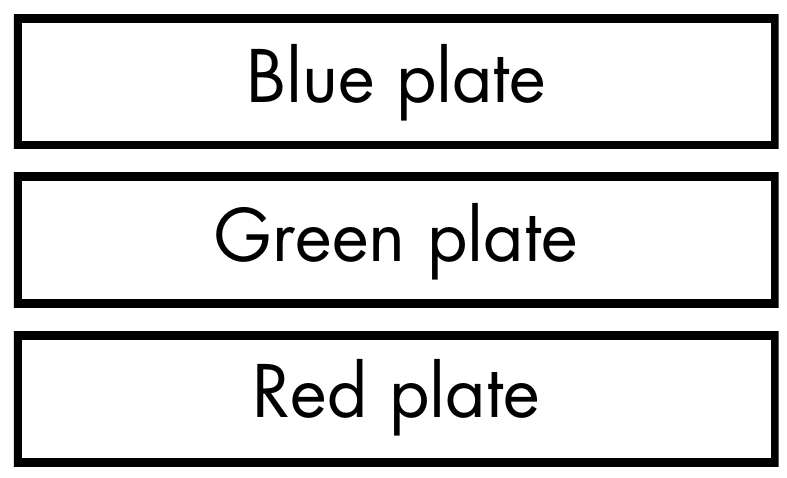
\includegraphics[width=0.5\textwidth]{img/fig11-1.png}
    \caption{Три обеденные тарелки в стопке}
    \label{fig11-1}
\end{figure}

4. Теперь проделайте операцию: вскройте кухонный прилавок. У нас будет синяя тарелка на кухонном столе (напомним, что синяя тарелка стояла на прикроватной тумбочке), а стопка обеденных тарелок останется такой, как показано на рисунке~\ref{fig11-2}.

\begin{figure}[htbp]
    \centering
    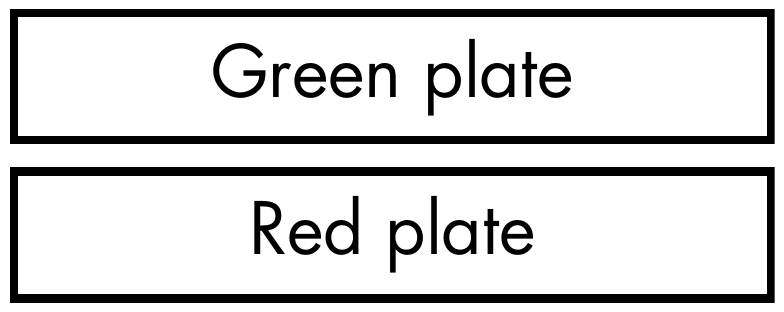
\includegraphics[width=0.5\textwidth]{img/fig11-2.png}
    \caption{Одна тарелка извлечена из стопки}
    \label{fig11-2}
\end{figure}

Если вы догадались, что действительно легко испортить стек, вы правы. Стек должен использоваться в соответствии со строгой дисциплиной. В любой функции:

\begin{itemize}
    \item Всегда помещайте элемент в стек, прежде чем что-либо извлекать.
    \item Никогда не высовывайте больше вещей, чем вы надели.
    \item Всегда выталкивайте все из стека.
\end{itemize}

Если вам не нужно извлекать элементы, вы можете просто настроить указатель стека. Это эквивалентно отбрасыванию элементов, которые выскочили. (Наша аналогия с обеденной тарелкой здесь не работает.)

Хороший способ поддерживать эту дисциплину — подумать об использовании скобок в алгебраическом выражении. Толчок аналогичен левой скобке, а всплывающий аналогичен правой скобке. Пары скобок могут быть вложены друг в друга, но они должны совпадать. Попытка поместить слишком много элементов в стек называется переполнением стека. Попытка вытолкнуть элементы из стека за пределы дна называется недостаточным заполнением стека.

Здесь мы рассмотрели только основные операции со стеком. Обычно в реализации стека добавляются другие операции. Например, операция просмотра позволяет просмотреть элемент на вершине стека, не удаляя его. И, как вы увидите в последующих главах, доступ к элементам, не находящимся на вершине стека, часто осуществляется напрямую, без добавления и извлечения, но очень хорошо контролируемым образом.

Стек реализуется путем выделения ему непрерывной области основной памяти. Стеки могут расти в любом направлении в памяти, в более высокие адреса или в более низкие. Восходящий стек растет до более высоких адресов, а нисходящий стек растет до более низких адресов. Указатель стека может указывать на верхний элемент в стеке, полный стек, или на место в памяти, где следующий элемент будет помещен в стек, пустой стек. Эти четыре возможные реализации стека показаны на рисунке~\ref{fig11-3} с целыми числами 1, 2 и 3, помещенными в стек в указанном порядке. Обязательно обратите внимание, что на этом рисунке адреса памяти увеличиваются вниз, как мы обычно видим их в отладчике \code{gdb}.

\begin{figure}[htbp]
    \centering
    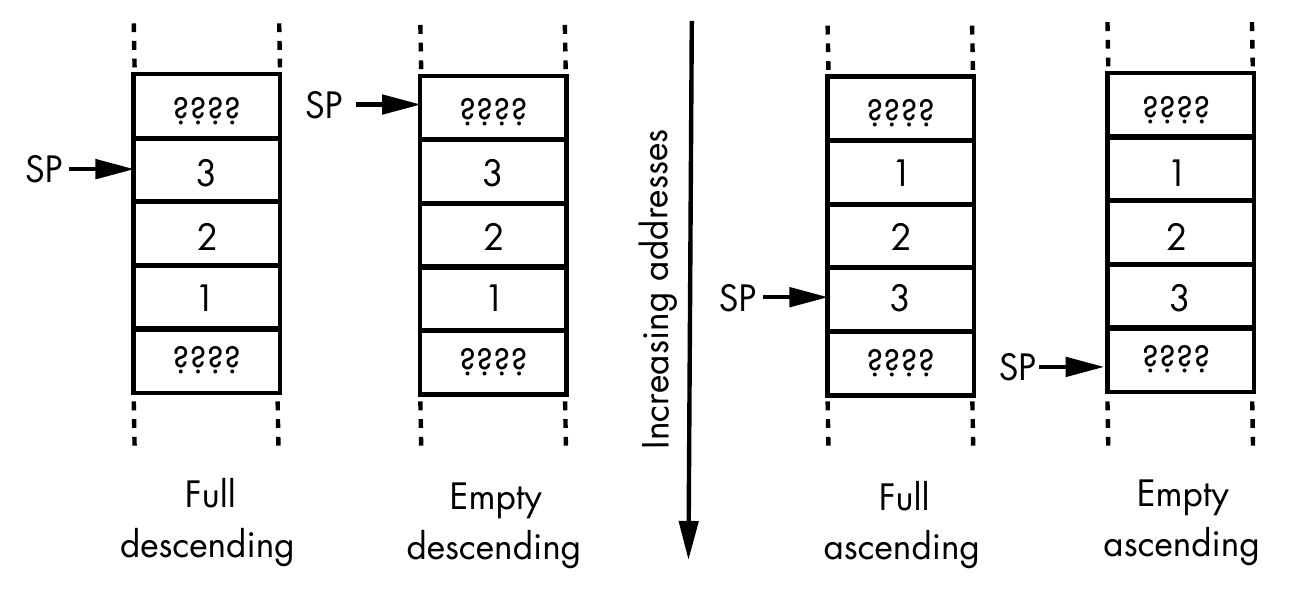
\includegraphics[width=0.9\textwidth]{img/fig11-3.png}
    \caption{Четыре способа реализации стека}
    \label{fig11-3}
\end{figure}

Инструкции x86-64 используют стек как полный нисходящий стек. Чтобы понять этот выбор, подумайте о том, как вы могли бы организовать вещи в памяти. Напомним, что блок управления автоматически увеличивает счетчик программ по мере выполнения вашей программы. Программы бывают самых разных размеров, поэтому хранение программных инструкций по низким адресам памяти обеспечивает максимальную гибкость в отношении размера программы.

Стек является динамической структурой. Вы не знаете заранее, сколько места в стеке потребуется той или иной программе во время ее выполнения. Невозможно узнать, сколько места выделить для стека. Вы хотели бы выделить как можно больше места, не допуская при этом его столкновения с инструкциями программы. Решение состоит в том, чтобы начать стек с наивысшего адреса и увеличивать его в сторону более низких адресов.

Это сильно упрощенное объяснение реализации стеков таким образом, чтобы они росли «вниз» в памяти. Организация различных элементов программы в памяти гораздо сложнее, чем простое описание, данное здесь. Но это может помочь вам понять, что есть несколько веских причин для того, что может показаться довольно странной реализацией.

Важным моментом является то, что нам нужно написать наш ассемблер соответствующим образом. Затем мы подробно рассмотрим, как стек используется в прологе и эпилоге функции, и как аргументы другой функции хранятся в регистрах, написав собственное «Hello, World!» программировать непосредственно на ассемблере.

\subsection{Внутри функции пролога и эпилога}

Моя версия на ассемблере «Hello, World!» Программа в листинге 11-3 очень похожа на язык ассемблера, сгенерированный из версии C компилятором в листинге 11-2, но я добавил комментарии и использовал более осмысленную метку для строковой константы. Это должно облегчить понимание того, как программа использует стек и передает аргументы функции записи.

\begin{ffcode}
# helloWorld.s
# Hello World program using the write() system call
        .intel_syntax noprefix
# Useful constant
        .equ    STDOUT, 1
# Constant data       
        .section  .rodata       
message:
        .string "Hello, World!\n"
        .equ    msgLength, .-message-1

# Code
        .text
        .globl  main
        .type   main, @function
main:
        push    rbp                 # save caller's frame pointer
        mov     rbp, rsp            # our frame pointer

        mov     edx, msgLength      # message length       
        lea     rsi, message[rip]   # message address
        mov     edi, STDOUT         # the screen
        call    write@plt           # write message

        mov     eax, 0              # return 0

        pop     rbp                 # restore caller frame pointer
        ret                         # back to caller
\end{ffcode}

\begin{center}
Листинг 11-3: «Привет, мир!» программа написана на ассемблере
\end{center}

Прежде чем мы перейдем к обсуждению пролога, обратите внимание, что я использовал другую директиву ассемблера, .equ, в листинге 11.3. (1). Формат следующий:

\begin{ffcode}
.equ symbol, expression
\end{ffcode}

Обратите внимание, что нам не нужно указывать сегмент .text для раздела .rodata (2). Ассемблер и компоновщик создают раздел .rodata, и операционная система сама определяет, куда его загрузить.

Выражение должно оцениваться как целое число, и ассемблер устанавливает символ, равный этому значению. Затем вы можете использовать этот символ в своем коде, что значительно облегчит его чтение, а ассемблер подставит значение выражения. Выражение часто представляет собой просто целое число. В этой программе я приравнял символ \code{STDOUT} к целому числу 1.

Cимвол <<\code{.}>> в выражении означает здесь место в памяти. Таким образом, когда ассемблер достигает выражения (3), он вычисляет текущую позицию в памяти, которая является концом текстовой строки в стиле C; вычитает начальное местоположение строки, место, которое программист пометил как сообщение, а затем вычитает 1 для завершающего символа NUL. Конечным результатом является то, что MsgLength приравнивается к количеству печатных символов в текстовой строке.

В главе 10 вы узнали, как указатель фрейма вызывающего объекта сохраняется в стеке вызовов и для этой функции устанавливается новый указатель фрейма. Но теперь, когда вы знаете больше о том, как работает стек вызовов, давайте пройдемся по прологу этой функции с помощью \code{gdb}.

Первое, что нам нужно сделать, это установить точку останова в начале функции:

\begin{ffcode}
    (gdb) b main
    Breakpoint 1 at 0x1139: file helloWorld.s, line 18.
\end{ffcode}

Вы можете использовать либо метку, либо основной, либо номер строки. Мы видели, как использовать команду \code{li} для просмотра номеров строк в главе 2. Использование номера строки может привести к тому, что \code{gdb} выполнит пролог и прекратит работу после него. (Я видел разное поведение в разных версиях \code{gdb}.)

После установки точки останова, когда мы запускаем программу, она прерывается на первой инструкции, и мы можем проверить содержимое регистров \code{rbp} и \code{rsp}:

\begin{ffcode}
    (gdb) r
    Starting program: /home/bob/progs/chap11/helloWorld_asm/helloWorld

    Breakpoint 1, main () at helloWorld.s:18
    18  push  rbp  # save caller's frame pointer
    (gdb) i r rbp rsp
    rbp  0x0  0x0
    rsp  0x7fffffffde88  0x7fffffffde88
\end{ffcode}

Команда \code{i r} дает нам текущее местоположение указателя стека, \code{rsp}. Инструкция, которая должна быть выполнена, поместит восемь байтов регистра \code{rbp} в стек вызовов. Чтобы увидеть эффекты в памяти, мы исследуем текущее содержимое стека. Поскольку стек вызовов полностью нисходящий, мы вычтем 8 из текущего адреса в указателе стека для нашего дисплея, чтобы мы могли получить представление об области памяти, которую эта инструкция изменит до того, как она изменится:

\begin{ffcode}
    (gdb) x/2xg 0x7fffffffde80
    0x7fffffffde80: 0x0000555555555160  0x00007ffff7de70b3
\end{ffcode}

Указатель стека в настоящее время указывает на значение 0x00007ffff7de70b3, которое является адресом возврата, который инструкция вызова в вызывающей функции (в среде выполнения C, поскольку это основная функция) помещается в стек. Регистр \code{rbp} содержит 0x0000000000000000. Это значение будет помещено в стек по адресу 0x7ffffffffde80, который в настоящее время содержит 0x00005555555555160.

Затем мы выполняем две инструкции в прологе функции, что приведет нас к первой инструкции после пролога:

\begin{ffcode}
    (gdb) si
    19  mov  rbp, rsp  # our frame pointer
    (gdb) si
    21  mov  edx, MsgLength  # message length
\end{ffcode}

Мы проверим значения в регистрах rsp и rbp:

\begin{ffcode}
    (gdb) i r rbp rsp
    rbp  0x7fffffffde80  0x7fffffffde80
    rsp  0x7fffffffde80  0x7fffffffde80
\end{ffcode}

...

\section{Локальные переменные в функции}

Переменные, определенные в функции C, могут использоваться в функции только там, где они определены, что делает их локальными переменными. Они создаются при вызове функции и удаляются, когда функция возвращается к вызывающей функции, поэтому их также называют автоматическими переменными.

В главе 9 вы узнали, что регистры ЦП можно использовать в качестве переменных, но если бы мы использовали регистры ЦП для хранения всех наших переменных, у нас скоро закончились бы регистры даже в небольшой программе, поэтому нам нужно выделить место в память для переменных.

Ранее мы также видели, что функция должна сохранять содержимое некоторых регистров (столбец «Сохранить?» в таблице 11.2) для вызывающей функции. Если мы хотим использовать такой регистр в нашей функции, нам нужно сохранить его содержимое в памяти и восстановить перед возвратом в вызывающую функцию.

Далее мы рассмотрим, как использовать стек вызовов для этих двух целей: создание и удаление автоматических переменных и сохранение и восстановление содержимого регистров.

\subsection{Переменные в стеке}

Из описания стека вызовов, показанного ранее, вы можете догадаться, что это хорошее место для сохранения содержимого регистра — просто поместите его в стек, прежде чем использовать регистр для чего-то другого, а затем извлеките содержимое из регистра перед возвратом в регистр. вызывающая функция.

Создание переменных в стеке вызовов более сложно. Если мы ограничим наше использование стека отправкой и извлечением, отслеживание того, где находится каждая переменная в стеке, быстро станет беспорядочной, если не невозможной.

Однако есть простой способ использовать стек для переменных. В рамках пролога функции мы выделим достаточно памяти для переменных в стеке, переместив указатель стека, тем самым увеличив размер кадра стека для функции. Мы можем использовать тот же метод адресации для доступа к нашим переменным в кадре стека, который использовался для доступа к адресу сообщения в листинге 11-3, за исключением того, что мы будем использовать указатель кадра, \code{rbp}, для базы адреса. Мы должны быть осторожны, чтобы не изменить \code{rbp}, чтобы мы могли использовать его в качестве контрольной точки во фрейме стека, оставляя указатель стека свободным для добавления и извлечения элементов по мере необходимости.

Чтобы проиллюстрировать, как использовать кадр стека для автоматических локальных переменных, мы начнем с программы на C в листинге 11.4, которая считывает один символ с клавиатуры и выводит его на экран.

\begin{ffcode}
/* echoChar.c
 * Echoes a character entered by the user.
 */

#include <unistd.h>

int main(void)
{
  char aLetter;

  write(STDOUT_FILENO, "Enter one character: ", 21); /* prompt user   */
  read(STDIN_FILENO, &aLetter, 1);                   /* one character */
  write(STDOUT_FILENO, "You entered: ", 13);         /* message       */
  write(STDOUT_FILENO, &aLetter, 1);

  return 0;
}
\end{ffcode}

\begin{center}
Листинг 11-4: Программа для отображения одного символа, введенного пользователем    
\end{center}


В листинге 11-5 показано, как это делает наш компилятор, представляющий собой язык ассемблера, который gcc генерирует для программы C в листинге 11-4.

\begin{ffcode}
	.file	"echoChar.c"
	.intel_syntax noprefix
	.text
	.section	.rodata
.LC0:
	.string	"Enter one character: "
.LC1:
	.string	"You entered: "
	.text
	.globl	main
	.type	main, @function
main:
	push	rbp
	mov	rbp, rsp
	sub	rsp, 16
	mov	rax, QWORD PTR fs:40
	mov	QWORD PTR -8[rbp], rax
	xor	eax, eax
	mov	edx, 21
	lea	rax, .LC0[rip]
	mov	rsi, rax
	mov	edi, 1
	call	write@PLT
	lea	rax, -9[rbp]
	mov	edx, 1
	mov	rsi, rax
	mov	edi, 0
	call	read@PLT
	mov	edx, 13
	lea	rax, .LC1[rip]
	mov	rsi, rax
	mov	edi, 1
	call	write@PLT
	lea	rax, -9[rbp]
	mov	edx, 1
	mov	rsi, rax
	mov	edi, 1
	call	write@PLT
	mov	eax, 0
	mov	rdx, QWORD PTR -8[rbp]
	sub	rdx, QWORD PTR fs:40
	je	.L3
	call	__stack_chk_fail@PLT
.L3:
	leave
	ret
	.size	main, .-main
	.ident	"GCC: (GNU) 12.1.1 20220730"
	.section	.note.GNU-stack,"",@progbits
\end{ffcode}

\begin{center}
Листинг 11-5. Язык ассемблера, сгенерированный компилятором для программы echoChar в листинге 11-4.
\end{center}

Программа на C определяет локальную символьную переменную \code{aLetter}, которая требует только один байт. Однако компилятор выделил 16 байтов в стеке вызовов, просто переместив указатель стека на 1. Архитектура x86-64 включает набор из шестнадцати 128-битных регистров, которые используются некоторыми инструкциями с плавающей запятой и векторами. Вы узнаете о них больше в главе 18. Для этих инструкций указатель стека должен быть выровнен по 16-байтовым границам адреса, поэтому в большинстве стандартов протоколов указано, что указатель стека должен быть выровнен по 16-байтовым границам. Это менее подвержено ошибкам, чем выравнивание указателя стека только там, где это необходимо.

Инструкция по перемещению указателя стека вводит инструкцию вычитания \code{sub}. Пока мы здесь, мы также опишем инструкции сложения и отрицания, сложения и отрицания.

...

Инструкции по умножению и делению более сложны и описаны в главе 16.

Нам нужно передать адрес локальной переменной \code{char} функции чтения, чтобы она могла сохранить там символ, введенный пользователем. Мы можем сделать это с помощью инструкции \code{lea} (загрузить эффективный адрес) (4). Как видите, компилятор выбрал байт, расположенный в 9 байтах внутри 16 байтов, выделенных в стеке. На рисунке~\ref{fig11-4} показано расположение этой переменной.

\begin{figure}[htbp]
    \centering
    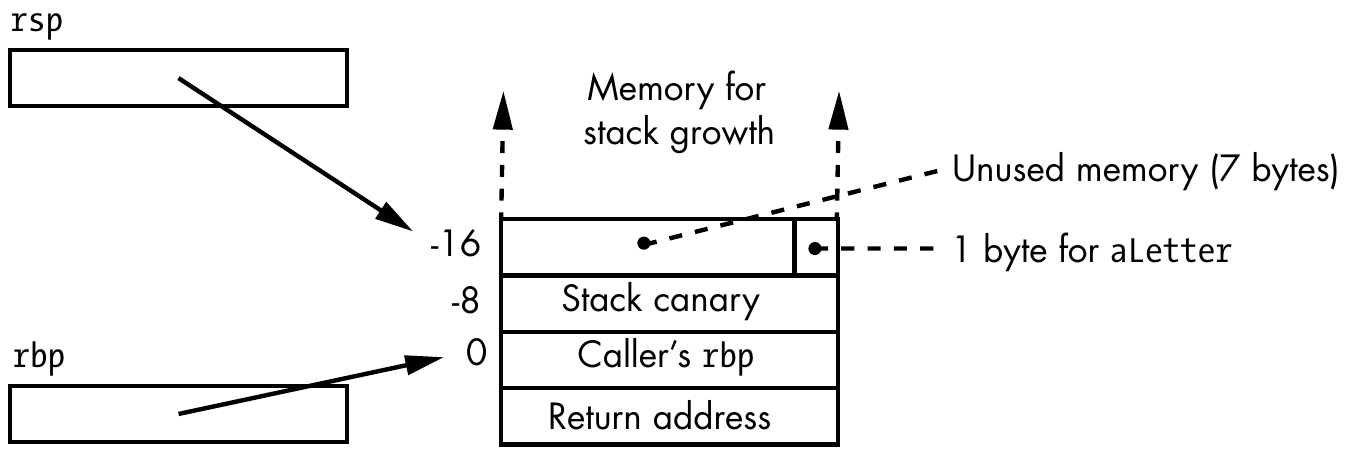
\includegraphics[width=0.9\textwidth]{img/fig11-4.png}
    \caption{Фрейм стека для программы в листинге 11-5}
    \label{fig11-4}
\end{figure}


Один из элементов кадра стека на рисунке~\ref{fig11-4} — это канарейка стека, которая используется для обнаружения повреждения стека.

\subsection{Повреждение стека}

Эпилог функции восстанавливает указатель фрейма вызывающего объекта в регистре rbp и возвращает указатель стека, указывающий на адрес возврата. Однако, если любое из этих значений было изменено в стеке, программа не будет вести себя должным образом. Канарейка стека может помочь определить, было ли изменено какое-либо из этих значений.

Когда программа запускается, операционная система сохраняет 64-битное случайное число в специальном месте памяти с пометкой \code{fs:40}, которое может изменить только операционная система. Мы читаем это значение из памяти (2) и сохраняем его во фрейме стека сразу после значения \code{rbp} (3) вызывающей программы. Затем, перед выполнением эпилога функции, мы проверяем, не изменилось ли значение стековой канарейки (5).

\textbf{Примечание.}
\textit{Использование стековой канарейки — необязательная функция. В моей версии \code{gcc} он используется по умолчанию. Вы можете переопределить поведение по умолчанию с помощью одного из параметров командной строки \code{-fstack-protector}, \code{-fstack-protector-strong} или \\ \code{-stack-protector-all}, чтобы использовать канарейку стека, и\\ \code{-fno-stack-protector}, чтобы не использовать ее.}

Код для выполнения этой проверки содержит еще две инструкции.

...

В листинге 11-5 код для проверки поврежденного стека 5 сначала извлекает значение, которое было сохранено в стеке, канареечный стек, а затем выполняет побитовое исключающее ИЛИ с исходным значением, которое было сгенерировано при первом запуске программы. в ячейке памяти \code{fs:40}. Если эти два значения идентичны, исключающее ИЛИ приводит к 0, что устанавливает флаг нулевого состояния \code{ZF} в 1 (истина), в результате чего инструкция \code{je .L3} переводит поток программы на инструкцию выхода, пропуская, таким образом, вызов функция \verb|__stack_chk_fail@PLT|. Если операция исключающее ИЛИ не возвращает 0, переход не произойдет, и программа вызовет функцию \verb|__stack_chk_fail@PLT|, которая сообщит об ошибке повреждения стека и завершит программу.

Вы видите еще одну новую инструкцию в этой программе, уходите.

...

Язык ассемблера, сгенерированный gcc в листинге 11.5, включает некоторые дополнительные обозначения \code{QWORD PTR 25}. В большинстве случаев ассемблер может вычислить размер операнда — байта, слова, двойного слова или четверного слова — из контекста инструкция. Если один из операндов является регистром, имя регистра определяет размер операнда. Но если один из операндов является адресом памяти, а другой — буквальной константой, размер операнда определить невозможно. Например, в листинге 11-5, если бы инструкция в 3 была следующей:

...

Давайте соберем все это воедино и напишем программу \code{echoChar} непосредственно на ассемблере. Мы будем использовать более осмысленные имена для меток, позволим ассемблеру вычислить длину текстовых строк и прокомментируем наш код, как показано в листинге 11.6.

\begin{ffcode}
# echoChar.s
# Prompts user to enter a character, then echoes the response
        .intel_syntax noprefix
# Useful constants
        .equ    STDIN,0
        .equ    STDOUT,1
# Stack frame
        .equ    aLetter,-9
        .equ    canary,-8
        .equ    localSize,-16

# Constant data
        .section  .rodata
prompt:
        .string "Enter one character: "
        .equ    promptSz,.-prompt-1
msg:
        .string "You entered: "
        .equ    msgSz,.-msg-1
        .text
# Code 
        .globl  main
        .type   main, @function
main:
        push    rbp                   # save caller's frame pointer
        mov     rbp, rsp              # our frame pointer
        add     rsp, localSize        # for local var.

        mov     rax, fs:40            # get stack canary
        mov     canary[rbp], rax      # and save it

        mov     edx, promptSz         # prompt size
        lea     rsi, prompt[rip]      # address of prompt text string
        mov     edi, STDOUT           # standard out
        call    write@plt             # invoke write function

        mov     edx, 1                # 1 character
        lea     rsi, aLetter[rbp]     # place to store character
        mov     edi, STDIN            # standard in
        call    read@plt              # invoke read function

        mov     edx, msgSz            # message size
        lea     rsi, msg[rip]         # address of message text string
        mov     edi, STDOUT           # standard out
        call    write@plt             # invoke write function

        mov     edx, 1                # 1 character
        lea     rsi, aLetter[rbp]     # place where character stored
        mov     edi, STDOUT           # standard out
        call    write@plt             # invoke write function

        mov     eax, 0                # return 0

        mov     rcx, canary[rbp]      # retrieve saved canary
        xor     rcx, fs:40            # and check it
        je      goodCanary
        call    __stack_chk_fail@PLT  # bad canary
goodCanary:
        mov     rsp, rbp              # delete local variables
        pop     rbp                   # restore caller's frame pointer
        ret                           # back to calling function
\end{ffcode}

\begin{center}
Листинг 11-6: Программа для отображения одного символа, написанная непосредственно на ассемблере
\end{center}

Читая код в листинге 11-6, я думаю, вы обнаружите, что присвоение имен смещениям для переменных в кадре стека значительно упрощает чтение кода. (1). Я также явно отменяю кадр стека вместо использования инструкции выхода. подчеркнуть происходящее (2).

В последующих главах вы узнаете, как использовать фрейм стека для более крупных и сложных переменных. Вы также узнаете, как использовать стек для передачи аргументов помимо шести, которые могут быть переданы в регистрах.

\section{Не использовать среду выполнения C}

Основная цель этой книги — показать, что происходит на уровне набора инструкций при написании на языках высокого уровня, поэтому мы продолжим использовать среду выполнения C (а позже и C++) и системный вызов записи и чтения POSIX. функции для оставшейся части этой книги.

Конечно, можно писать автономные программы, не использующие среду выполнения C. Вы увидите, как это делается, в главе 20.

...
